\subsection{Robot}
\label{sub:robots}
Gli agenti che modellano il comportamento dei robot sono, di fatto, la componenete principale di tutto il sistema.
Sono i robot, e loro soltanto, a muoversi all'interno del territorio cercando i feriti e costruendo, nel mentre, la rete \textit{mesh}. 
Nonostante abbiano un ruolo così fondamentale, questi agenti sono a tutti gli effetti dei \textit{reflexive agent with internal state} facendo riferimento alla classificazione proposta da Russell e Norvig \cite{russell2016}, il cui comportamento viene descritto di seguito.
È bene esplicitare, prima di proseguire, qual è lo stato interno dell'agente descritto: in questo caso, lo stato interno è dato da un insieme di variabili, in particolare:
\begin{itemize}
	\item \texttt{target\_cell}, ovvero la cella di frontiera a cui il robot è diretto;
	\item \texttt{target\_path} è il cammino minimo che l'agente deve seguire per raggiungere la cella obiettivo dalla posizione attuale;
	\item \texttt{status} serve per indicare se il robot sta esplorando una cella, si sta muovendo, sta scegliendo la prossima cella obiettivo (o sta aspettando che nuove celle si aggiungano alla frontiera) oppure che si è rotto.
\end{itemize}
Per alleggerire la lettura del diagramma di flusso sottostante e per comodità di descrizione dell'agente la casistica del fallimento di un robot verrà descritta di seguito separatamente.
Inoltre, come già detto nella Sezione \ref{sec:environment}, questi agenti presentano un insieme di altre variabili che ne descrivono delle caratteristiche o che vengono sfruttate dall'agente per effettuare delle scelte a livello “microscopico” (\textit{e.g.}, quale cella scegliere come obiettivo); a queste si aggiungono tra ulteriori variaibli di interesse: la posizione in cui si trova l'agente, quella precedente e l'utilità della cella scelta come obiettivo prima che venisse modificata (variabile utilizzata per la gestione dei fallimenti dei robot).
Infine, a livello programmativo, sono presenti un insieme di variaibli atte a simulare il tempo che il robot trascorre per spostarsi da una posizione ad un'altra o per esplorare una cella. 

Durante la sua vita\margin{Comportamento dell'agente}, l'agente valuta il suo stato interno e se sta mantenendo una connessione con la rete \textit{mesh} oppure no, in base a queste due condizioni prende delle decisioni “macroscopiche” su quali azioni effettuare (\textit{e.g.}, decide di rilasciare un ripetitore \textit{wi-fi} oppure di continuare a muoversi verso l'obiettivo) come mostrato in Figura \ref{fig:robotworkflow}.
È importante far notare che il processo decisionale non avviene ad ogni \textit{step} della simulazione (cioè ad ogni secondo d'orologio), ma solo quando lo stato interno del robot subisce delle modifiche.
\begin{figure}
	\centering
	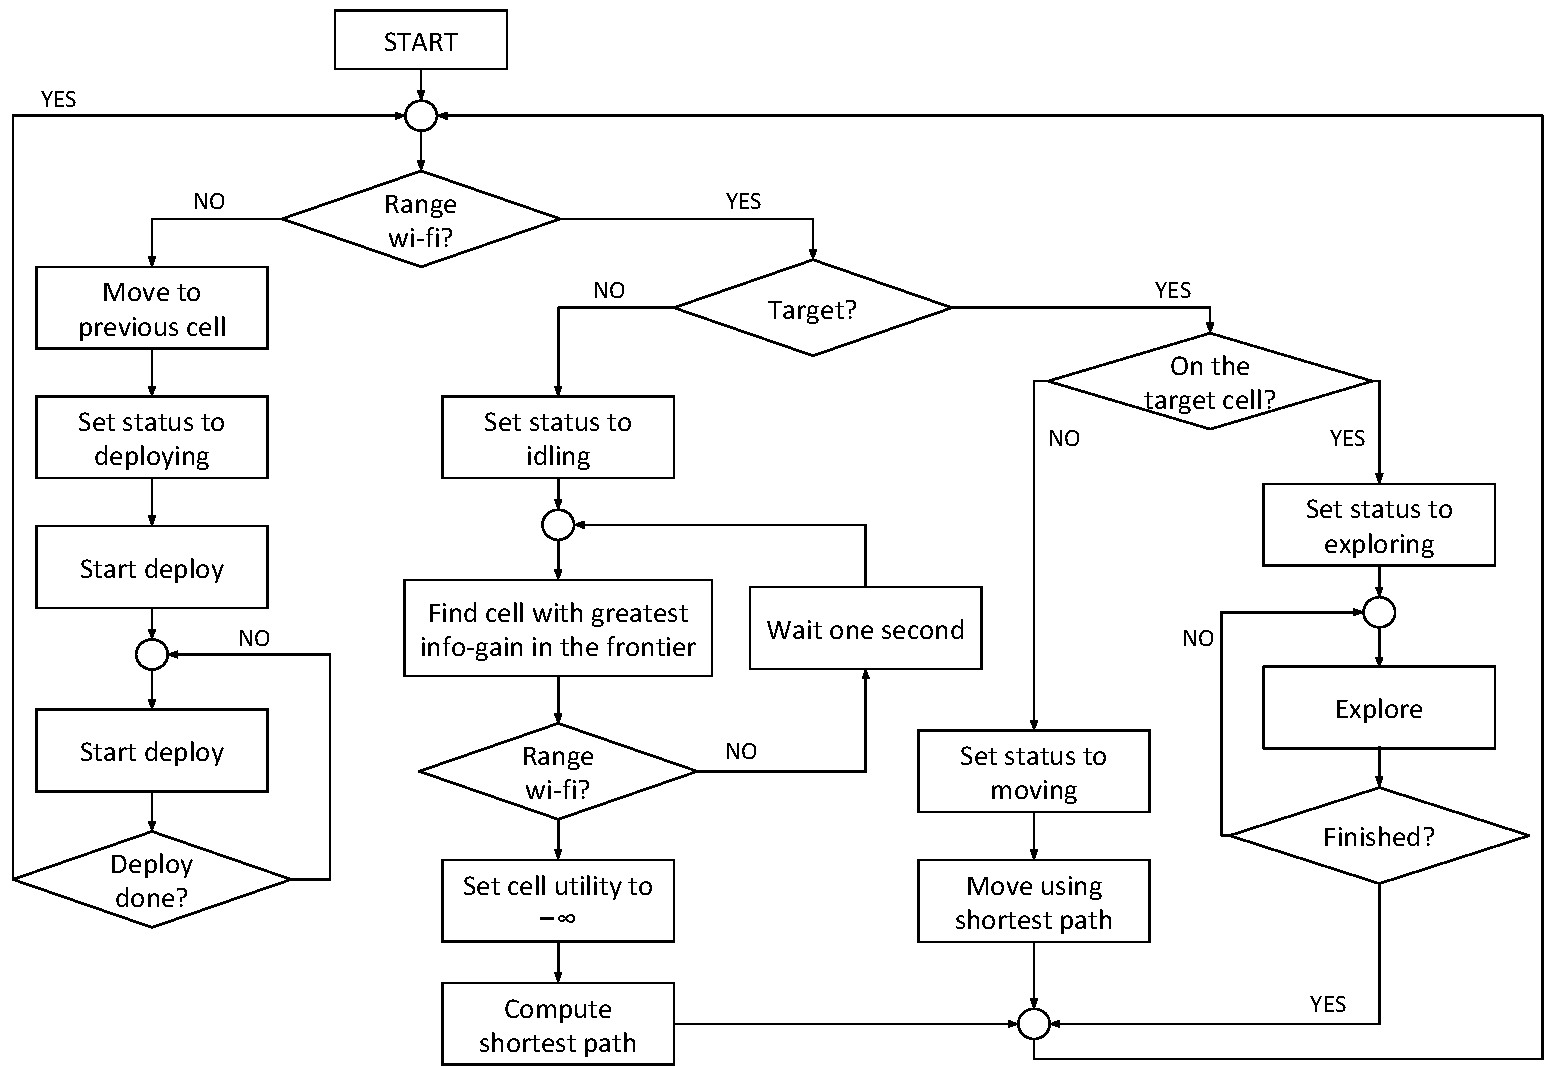
\includegraphics[width=1.0\linewidth]{images/Robot_workflow}
	\caption{Figura che rappresenta il processo decisionale che l'agente robot effettua quando deve stabilire la sua prossima azione, tale processo si basa sullo stato interno del robot e sulla presenza (o assenza) di connessione con la rete \textit{mesh}; si noti, che quello appena descritto non avviene ad ogni step della simulazione ma solo quando lo stato interno dell'agente subisce dei cambiamenti.}
	\label{fig:robotworkflow}
\end{figure}
Per prima cosa, il robot valuta se è ancora all'interno della copertura \textit{wi-fi} poiché, per come è stato definito il metodo di comunicazione e coordinamento dei robot, risulta fondamentale che siano sempre in grado di comunicare tra loro.
Tale controllo risulta essere necessario farlo ogni volta che il robot si sposta di una cella, perché è l'unico caso in cui si suppone che l'agente possa perdere la connessione uscendo dall'area coperta; per comodità e “pulizia” algoritmica viene anche effettuato nel caso in cui il robot ha finito di esplorare una cella.
Quando il robot, muovendosi, esce dalla zona coperta, se ne accorge e allo \textit{step} successivo rientra immeditamente nella zona coperta iniziando il processo di rilascio del \textit{bean}: aggiorna il suo stato in fase di \textit{deploy}, iniziando poi il processo di rilascio il quale abbiamo supposto impieghi circa 15 secondi (\textit{i.e.}, 15 \textit{step}) poiché il rilascio del ripetitore deve essere effettuato in un luogo e in modo sicuro.\\
Altrimenti, se il robot è in una zona coperta, la sua decisione viene determinata dal possedimento di una cella \textit{target}.
In particolare, se non possiede una cella obiettivo deve sceglierne una: per prima cosa, si mette in stato di \textit{idling}, ovvero lo stato indicante che il robot è fermo per calcolare il suo prossimo obiettivo oppure che non ha celle tra cui scegliere.
In seguito, deve stabilire la cella “migliore” da esplorare; per far ciò, i robot sfruttano un concetto di \textit{information gain} (o \textit{info-gain}), \todo[inline]{qua mi sa che c'è da citare l'articolo dicendo cosa noi abbiamo cambiato rispetto a loro, puoi farlo te? Grazie DP} il quale è uno scalare che indica “quanta informazione può portare l'esplorazione di una cella”, ovvero più tale valore è alto più ad un agente conviene andare ad esplorare tale cella.
La Formula \ref{math:info-gain} è quella utilizzata dagli agenti per il calcolo dell'\textit{info-gain}, tale valore viene calcolato per ogni cella della frontiera.
\begin{equation}
	\label{math:info-gain}
	\textit{Information gain} = \rho+\mu-\alpha\omega
\end{equation}
In tale formula:
\begin{itemize}
	\item $\rho$ è la priorità della cella che risulta essere pari a zero tranne nei casi in cui la cella sia adiacente ad una cella in cui una vittima sia riuscita a segnalare la sua presenza;
	\item $\mu$ è l'utilità della cella;
	\item $\alpha$ è il parametro, già nominato in precedenza, che indica quanto il costo del percorso per raggiungere la cella d'interesse pesi nella scelta, più il valore è alto più ci si aspetta che il costo influisca in maniera significativa e viceversa, ovvero valorizzando di più l'utilità e la priorità delle celle ma non il costo per raggiungerle;
	\item $\omega$ è il costo, in termini di \textit{step} necessari per raggiungere la cella d'interesse. 
\end{itemize}
Si sottolinea che per il calcolo di $\omega$ per ogni cella della frontiera, viene computato il costo del cammino minimo sfruttando la rappresentazione interna del territorio che possegono (e condividono) i robot sotto forma di grafo; \textit{i.e.}, si calcolano precedentemente al calcolo dell'\textit{info-gain} tutti i cammini minimi (e i loro costi) dalla cella in cui è presente il robot verso tutte le altre celle sfruttando l'algoritmo definito da Dijkstra.
Una volta computato l'\textit{info-gain} per ogni cella, l'agente sceglie quella con il valore maggiore tra tutte le celle della frontiera, diventando così la cella \textit{target} dell'agente.
Se il robot è riuscito ad individuare la sua prossima cella obiettivo, imposta l'utilità di tale cella pari a $-\infty$ in modo che nessun altro agente scelga tale cella, memorizza il cammino minimo da intraprendere e poi \textit{rimuove la cella dalla frontiera}.\todo[inline]{perché la rimuoviamo in find best cell la cella dalla frotniera? non dovremmo rimuoverla quando il robot la esplora? per come abbiamo definito la frontiera quella cella è ancora in frontiera, come lo sistemiamo nella relazione? giustificando quello che abbiamo scritto nel codice? Il tappeto può essere una soluzione? DP}
Infine, il robot, \textit{quando arriva nella cella obiettivo}, diminuisce l'utilità di tutte le celle del vicinato di \textit{Moore} che riesce a percepire sfruttando i suoi sensori e che sono effettivamente nella linea “visiva” del robot; tutte le celle che sarebbero visibili dai sensori del robot, ma che non possono venir percepite per via delle macerie (ovvero le celle con valore di \texttt{explored} pari a $-1$) che ne ostacolano la visione, non subiscono tale diminuzione di utilità.
La formula di riduzione dell'utilità utilizzata risulta essere differente rispetto a quella proposta nel principale lavoro di riferimento \cite{burgard2005}, ma il principio risulta lo stesso: più la cella è vicina al robot più la sua utilità viene diminuita in modo che gli agenti lontani da essa siano meno invogliati a muoversi in quella direzione.
La riduzione dell'utilità è definita dalla Formula \ref{math:utility-red}; la differenza rispetto all'articolo è che la riduzione proposta veniva effettuata mediante una sottrazione che può portare a valori negativi dell'utilità, dato che tale proposta non ha convinto appieno in termini di “eleganza”, si è optato per una soluzione che sfrutta lo stesso principio ma non rende negativa l'utilità. \todo[inline]{Eviterei una supercazzola lunga tre pagine. Sicuramente è da sistemare l'italiano, ma spero anche che tu ti ricorda perché hai mosso tali obiezioni sulla loro sottrazione DP}
\begin{equation}
	\label{math:utility-red}
	\mu = \mu\times\gamma\left(\frac{\textbf{d}}{\textbf{r}}\right)
\end{equation}
Come in precedenza, $\mu$ è l'utilità della cella, \textbf{d} è la distanza tra le due celle definita come numero di celle da attraversare per raggiungere la destinazione, siano esse celle sugli assi, diagonali o entrambe; invece, \textbf{r} è il raggio di percezione del robot.
Infine, $\gamma$ (valore che varia nell'intervallo $\left[0, 1\right]$) stabilisce, di fatto, quanto l'utilità deve venir effettivamente diminuita per il rapporto tra la distanza e il raggio di percezione. 
Qualitativamente, ci si aspetta che quando $\gamma$ è piccola, l'utilità diminuisce in fretta e quindi i robot tenderanno a mantenersi distanti tra loro; al crescere del parametro i robot potrebbero tendere a rimanere più vicini poiché vi sarebbero celle con utilità elevata anche nelle vicinanze di altri agenti.
Quindi, ad alcuni robot potrebbe risultare conveniente scegliere delle celle con utilità maggiore ma più distanti, si tenga, comunque, presente il metodo di selezione basato sul concetto di \textit{info-gain} e la Formula \ref{math:info-gain}.
\todo[inline]{Anche questa riduzione non sarebbe da fare una volta che il robot arriva sulla cella e percepisce attorno? Perché nel codice sfruttiamo la lof ma il robot è ancora nella cella di partenza quando usa find best cell DP}
\todo[inline]]{Perché proprio diviso il radar radius? Puoi aggiungerlo te? Grazie DP}
Vi sono dei casi in cui è possibile che l'agente non riesca a stabilire il suo prossimo obiettivo perché non vi sono celle nella frontiera oppure perché tutte le celle hanno utilità pari a meno infinito e quindi stanno già venendo esplorate da un altro robot; in questi casi, i robot aspettano un secondo prima di riaggiornare la rappresentazione del territorio condivisa e cercando nuovamente una possibile cella.\\
Se invece il robot possiede una destinazione, deve verificare se ha raggiunto la posizione designata: se non vi è ancora arrivato continua a muoversi seguendo il cammino minimo, calcolato in precedenza, e aggiorna la sua ultima posizione e quella attuale.
Si noti che durante il processo di movimento il robot continua a verificare di essere ancora all'interno della copertura del segnale, se ciò non avviene, incomincia la fase di rilascio del ripetitore per poi riprendere a muoversi sfruttando il cammino minimo calcolato in precedenza.
\todo[inline]{È davvero necessario che diciamo che il cammino è salvato in una coda e che ogni volta che si passa da una cella all'latra si rimuove la coordinata e poi se ci si mette in deploy il rimanente della coda rimane ecc ecc.? DP}
Invece, se è nella cella designata l'agente modifica il suo stato e inizia la \textit{routine} di esplorazione.\\
Una volta finita l'esplorazione, tutto il processo appena descritto viene ripetuto nuovamente

Fin'ora è stato dato per scontato\margin{Comunicazione tra gli agenti} come i robot comunichino tra loro.
Nonostante la completezza dei meccanismi di comunicazione non sia stata implementata direttamente all'interno del simulatore, poiché è stato considerato un problema che esulasse dagli obiettivi del lavoro, teniamo a voler sottolineare come abbiamo pensato in linea teorica il meccanismo di comunicazione e quindi perché sono state utilizzate delle “semplificazioni” programmative a livello di simulatore.
L'idea principale del metodo proposto è che i robot mentre esplorano costruiscono la rete \textit{mesh} che non solo permette ai feriti di segnalare la loro posizione mediante l'utilizzo del GPS, ma permette anche ai robot di sfruttarla per comunicare tra loro come con qualsiasi rete \textit{wi-fi}.
Di conseguenza, per come è stato proposto il meccanismo della rete \textit{mesh} \textit{citare il paper di cui non mi ricordo il nome} che richiede la presenza di un ripetitore madre, si è pensato che tale ripetitore (o un pc ad esso collegato) possa tenere in memoria l'insieme delle coordinate GPS che rappresentano la frontiera e la rappresentazione della mappa del territorio che sta venendo esplorato dai robot: una rappresentazione a grafo analoga al \texttt{seen\_graph} descritta nella Sezione \ref{sec:environment}.
Ovvero, ogni nodo rappresenta una cella, in particolare un'area di 3$\times$3 metri indicata da una coordinata GPS ricadente in tale area; gli archi rappresentano i passaggi possibili da un'area ad un'altra con un peso che indica la difficoltà stimata di attraversamento, tale difficoltà è stabilita dalla difficoltà della cella indicata dal nodo sorgente dell'arco.
In questo modo, i robot hanno tutte le informazioni rilevanti: quali celle sono state viste (i nodi del grafo) e la loro difficoltà stimata di attraversamento (il peso degli archi) e quali sono le celle appartenenti alla frontiera.
Poiché i robot si garantiscono di essere sempre nelle copertura della rete, ogni volta che devono comunicare qualcosa (\textit{i.e.}, la vista effettiva del territorio in nuove coordinate oppure il ritrovamento di un ferito) o prendere una qualche decisione (\textit{i.e.}, la prossima cella obiettivo) prima richiedono la versione aggiornata di tali dati e poi comunicano le eventuali novità scoperte o aggiornano dei valori all'interno della rappresentazione del territorio.
Tali comunicazioni, come già detto, sono state rese trasparenti poiché le riteniamo un problema più tecnico e di poco costo temporale rispetto alla scala considerata nel lavoro; di conesguenza, è stata preferita una rappresentazione a livello programmativo di tali dati direttamente nella classe che descrive l'ambeinte (come già detto) e quindi direttamente condivisa tra tutti gli agenti.

\todo[inline]{Potresti scriverci te due righe così evito di scrivere cose completamente confuse che poi saranno da sistemare? Grazie DP P.S. guarda anche il commento in injured.py che da una parte in sos high stai facendo una moltiplicazione che fa zero sempre.}
\margin{Metodologie di prioritizzazione}
\todo[inline]{fallimenti parlarne altrove? DP}

\todo[inline]{Non li ho scritti da nessuna parte, dobbiamo parlarne ma non ho idea dove. DP}
\subsection{Ferito}
Questo agente rappresenta le persone ferite che sono disperse nell'area di interesse e necessitano di essere individuate e salvate, si noti che il loro salvataggio non fa parte di questo simulatore poiché le metodologie di salvataggio dipendono da troppi fattori che non possono venir considerati complessivamente in un simulatore (\textit{e.g.}, la loro possibilità di muoversi oppure se richiedono un intervento medico sul campo).
Il loro comportamento è stocastico ma basato su uno stato interno, di conseguenza tali agenti sono stati classificati come \textit{reflexive agent with internal state}, facendo nuovamente riferimento alla classificazione proposta da Russell e Norvig \cite{russell2016}.
L'agente è molto semplice, possiede due attributi che lo descrivono: la posizione all'interno della griglia e lo stato interno; lo stato assume valore 0 nel momento in cui non è ancora stato trovato e 1 quando è stato trovato e quindi salvato successivamente.
Il suo comportamento, come detto, dipende dal suo stato interno, in particolare: 
\begin{itemize}
	\item finché tale agente non è stato individuato e la cella in cui si trova non è coperta dal \textit{wi-fi} non fa nulla;
	\item se si trova in una cella coperta e non è ancora stato individuato, ha una probabilità pari a $10^{-3}$ di segnalare la sua presenza collegandosi alla rete \textit{mesh}, tale probabilità risulta essere bassa perché bisogna considerare che ad ogni \textit{step} (un secondo di tempo d'orologio) della simulazione un ferito può segnalare la sua presenza ed inoltre non tutte le persone potrebbero aver accesso ad un telefono in una situazione critica;
	\item se è stato individuato da un robot o ha già segnalato la sua presenza, non fa altro che aspettare.
\end{itemize}
% Le due metodologie di prioritizzazione dei feriti le nasconderei sotto il cappuccio e ne parlerei nei robot DP